% Chapter 1

\chapter{Photon calibrator} % Main chapter title

\label{Chapter1} % For referencing the chapter elsewhere, use \ref{Chapter1} 

%----------------------------------------------------------------------------------------

% Define some commands to keep the formatting separated from the content 


%----------------------------------------------------------------------------------------

\section{Photon calibrator}
Photon calibrator relies on photon radiation pressure from auxiliary 
power-modulated laser beams reflecting on the test mass to apply periodic 
forces via the recoil of photons. Controlling and measuring the laser power 
accurately is one of the principal challenges of Pcal development. 
The KAGRA Pcal system consists of transmitter module, in-vacuum periscope, 
Receiver module and Beam monitor system. The transmitter module accurately 
modulates the beam power with internal feedback loop called optical follower 
servo. Two laser beams from the transmitter module enter the vacuum enclosure 
and relayed by mirrors mounted to a periscope structure located inside the 
vacuum envelope, then impinge on the test mass mirror to apply forces. 
The reflected beams are relayed exactly in the symmetric path by the 
other set of mirrors mounted to the periscope and enter the receiver module. 
Capturing the beams reflected from the test mass is important to ensure 
that the applied power is exactly same as modulated without losing 
somewhere in the beam path.

An important aspect of the performance of the Pcal system is the locations 
of the beam spots on the test mass surface. The photon pressure forces can 
induce both local and bulk elastic deformations of the test mass which 
compromise the accuracy of the calibration. To minimize the impact of these 
deformations, Pcal uses two beams displaced symmetrically from the center 
of the face of the test mass mirror. In order to determine and adjust the 
positions of the Pcal beams, the beam position monitor system will be 
installed. It consists of remote-controlled digital camera, telescope and 
relay mirrors. It will also provide monitoring of the surface condition of 
the test mass mirror as well as the change of the test mass mirror position 
during the cooling down phase.

%One of the goals of the gravitational wave experiment is the accurate measurement of the gravitational waveform that is measured through the absolute displacement of the end test masses. A recent study that LIGO conducted in US showed that a displacement uncertainty could be controlled  by the photon calibrator. The photon calibrator is one of the calibration tools to push the mirror surface using the photon pressure of the laser as shown in Fig XXX.

The absolute displacement is described as
\begin{equation}
dx=\frac{P \cos{\theta}}{c} s(f) \left( 1+\frac{I}{M}\vec{a}\cdot \vec{b}\right), \label{eq:dx}
\end{equation}
where $P$ is an absolute power of the laser, $c$ is the speed of light, $\theta$  is an incident angle of the laser, $I$ and $M$ are moment of inertia and mass of test mass, $\vec{a}$ and $\vec{b}$ is position vector of photon calibrator lasers and interferometer laser. Then, $s(f)$ is transfer function of the test masses. We simulated the transfer function of test mass as shown in Fig. XXX. We assumed the masses, shapes and Young's modules of the each pendulum mass and fiber as shown in Fig.XXX. According to transfer function, we can regard the motion of high frequency as free mass due to higher than the natural frequency. Therefore, we are able to assume as follows:
\begin{equation}
s(f)=\frac{1}{M \omega^2},
\end{equation}
where $\omega$ is the angular frequency of test mass.
 
%----------------------------------------------------------------------------------------

\section{Purpose of photon calibrator}
\subsection{Interferometer Calibration}

One of the main calibration method to reconstruct $\Delta L_{\rm ext}$, differenctial arm length (DARM), 
uses the combination of obtained error signal($d_{\rm err}$) and feedback signal($d_{\rm ctrl}$) 
with considering the slow temporal variations in aLIGO
\footnote{The detail document is https://arxiv.org/pdf/1608.05134.pdf}. 
In this document, we assume the LIGO DARM control system which is shown in Figure~\ref{fig:L_DARM_control_loop}
({\bf Ask experts how to control in bKAGRA, especially Actuator part}). 
\begin{figure}
\begin{center}
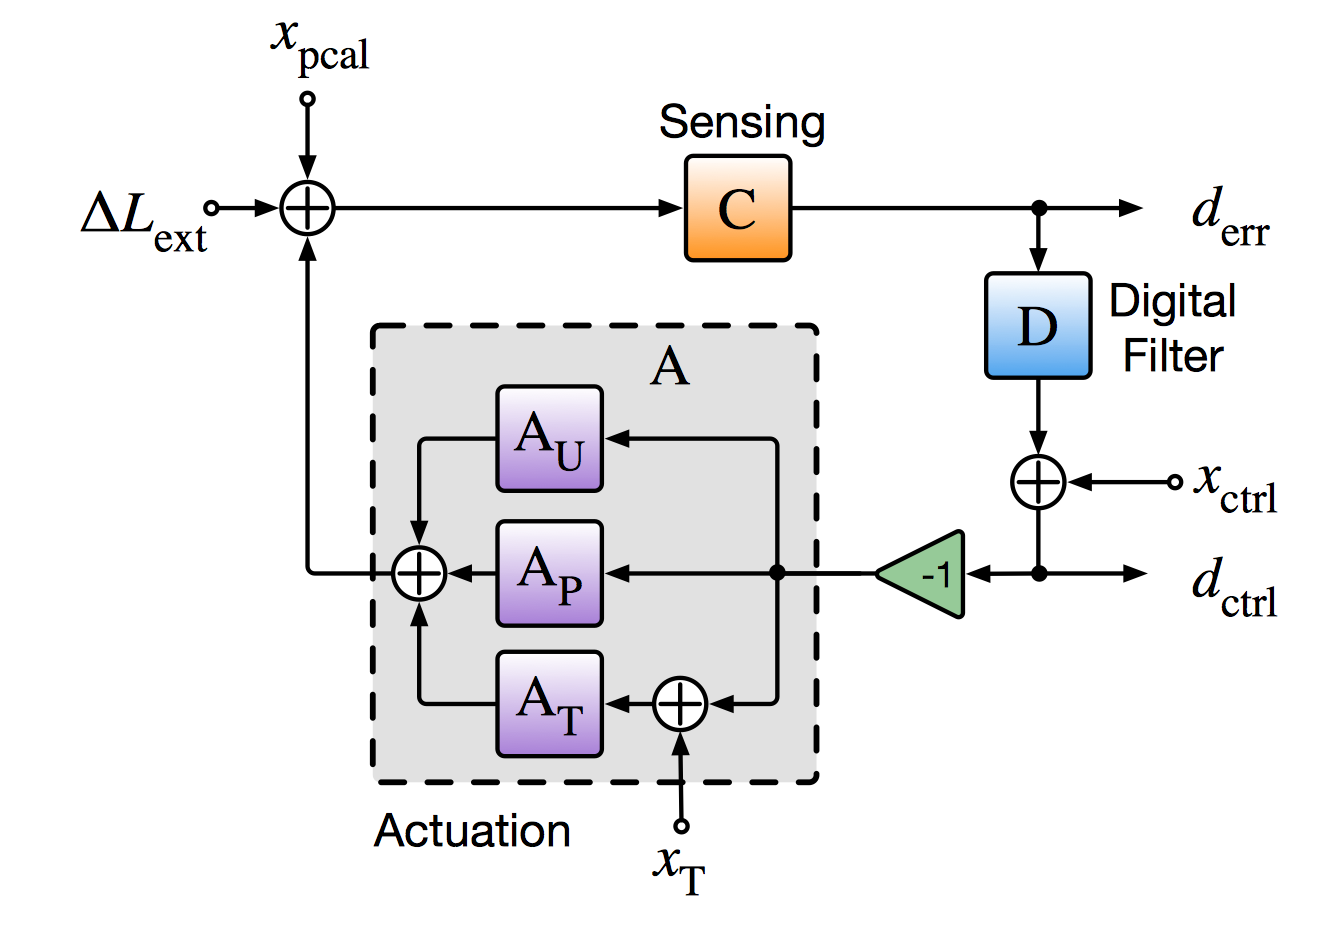
\includegraphics[width=8cm]{Figures/L_DARM_control_loop.eps}
\caption{Schematic diagram of the LIGO DARM control loop.}
\label{fig:L_DARM_control_loop} 
\end{center}
\end{figure}
This servo is described in term of 
(i) sensing function, $C(f,t)$ 
(ii) digital filters, $D(f)$ 
(iii)actuation function, $A(f,t)$, 
and $G(f,t) = C(f,t)D(f)A(f,t)$ is the DARM open loop transfer function  

The sensing function$C(f,t)$ can be written in
\begin{equation}
C(f,t) = \frac{\kappa_{\rm C}(t)}{1+if/f_{\rm C}(t)}Q(f) \equiv P(f,t) Q(f).
\end{equation}
$Q(f)$ is the time-independent part of the sensing function, which includes
photodetector response,
electronic response
and signal delay caused by light traveling time of interferometer arm.
$P(f,t)$ is the time-dependent part of the sensing function, which includes
optical gain sale factor, $\kappa_{\rm C}(t)$ and coupled-cavity response.
Coupled-cavity response is approximated by a single pole ($f_{\rm C}(t)$).

The actuation function$A(f,t)$ can be written in
\begin{equation}
A(f,t) = \kappa_{\rm PU}(t)(A_{\rm P,0}(f)+A_{\rm U,0}(f)) + \kappa_{\rm T}(t) A_{\rm T,0}(f).
\end{equation}
$A_{\rm P,0}(f)$, $A_{\rm U,0}(f)$ and $A_{\rm T,0}(f)$ are models of the actuation function 
of the penultimate, upper-intermediate and the test mass stage 
when both $\kappa_{\rm PU}(t_0)$ and $\kappa_{\rm T}(t_0)$ are set to 1.

To monitor those four time variation parameters, 
$\kappa_{\rm C}(t)$, $f_{\rm C}(t)$, $\kappa_{\rm PU}(t)$ and $\kappa_{\rm T}(t)$, 
we need to inject modulated excitations into the DARM loop.
Also, to measure the $\kappa_{\rm C}(t)$ individually form $\kappa_{\rm PU}(t)$ and $\kappa_{\rm T}(t)$,
we need additional system to inject modulated excitations to ETM.
Photon calibrator is powerful tool for this purpose.
So, we should inject following four modulated excitations;
(i) two modulated excitations using a photon calibrator system ($x_{\rm pcal1}$ and $x_{\rm pcal2}$)
(ii) one modulated excitations into the overall DARM actuation ($x_{\rm ctrl}$)
(iii) one modulated excitations into the test mass stage actuation ($x_{\rm T}$).
The responses in $d_{\rm err}$ at time $t=t'$ for each modulated excitations can be written by
\begin{eqnarray}
d_{\rm err, t'}(f_{\rm pcal1}) &=& \frac{C(f_{\rm pcal1},t')}{1+G(f_{\rm pcal1},t')} x_{\rm pcal1} \\
d_{\rm err, t'}(f_{\rm pcal2}) &=& \frac{C(f_{\rm pcal2},t')}{1+G(f_{\rm pcal2},t')} x_{\rm pcal2} \\
d_{\rm err, t'}(f_{\rm ctrl}) &=& \frac{-A(f_{\rm ctrl}, t')C(f_{\rm ctrl},t')}{1+G(f_{\rm ctrl},t')} x_{\rm ctrl}  \\
d_{\rm err, t'}(f_{\rm T}) &=& \frac{\kappa_{\rm T}(t') A_{\rm T,0}(f_{\rm T}, t')C(f_{\rm T},t')}{1+G(f_{\rm T},t')} x_{\rm T} 
\end{eqnarray}
Using $x_{\rm pcal1}$ and $x_{\rm T}$ modulated excitations, $\kappa_{\rm T}(t')$ is obtained.
Using $x_{\rm ctrl}$ modulated excitation and $\kappa_{\rm T}(t')$, $\kappa_{\rm PU}(t')$ and $A(f,t')$ are obtained. 
Using $x_{\rm pcal2}$ modulated excitation and $A(f,t')$, $\kappa_{\rm C}(t')$ and $f_{\rm C}(t')$ are obtained.

Finally, $\Delta L_{\rm ext}(t)$ is reconstructed by following equation:
\begin{eqnarray}
\Delta L_{\rm ext}(t) = &[{\cal P}(f_{\rm C}(t))/ \kappa_{\rm C}(t) * {\cal Q} ] * d_{\rm err}(t) \nonumber \\
& + [ 
  \kappa_{\rm PU}(t)({\cal A}_{\rm P,0} + {\cal A}_{\rm U,0}) + \kappa_{\rm T}(t) {\cal A}_{\rm T,0}  
]
* d_{\rm ctrl}(t),
\end{eqnarray}
where ${\cal P}(f_{\rm C}(t))$, ${\cal Q}$, ${\cal A_{\rm P,0}}$, ${\cal A_{\rm U,0}}$ and ${\cal A_{\rm T,0}}$  
are the time-domain filters created from $P(f,t)$, $Q(f)$, $A_{\rm P,0}(f)$, $A_{\rm U,0}(f)$ and $A_{\rm T,0}(f)$, and $*$ denotes convolution.

To reduced the systematic uncertainty, frequencies of modulated excitations are selected with following conditions:
(1) Frequencies of $x_{\rm pcal1}$ , $x_{\rm ctrl}$ and $x_{\rm T}$ should be in a narrow frequency band.
(2) Such frequency band should be selected where the magnitude of the transfer functions of 
the combined penultimate and upper intermediate mass stage and the test mass stage are 
approximately equal.
(3) Frequencies of $x_{\rm pcal2}$ should be near the coupled-cavity pole frequency.


\subsection{Hardware injection test}
\subsection{Photon pressure actuator}

%----------------------------------------------------------------------------------------

\section{Calibration line of KAGRA}


%----------------------------------------------------------------------------------------

